\chapter{Vũ trụ Newton đang giãn nở}

\lectureoverview{Vũ trụ học hiện đại bắt đầu khi bản thân vũ trụ được xem như một hệ vật lý. Xuất phát từ tính đẳng hướng và đồng nhất ở quy mô lớn, ta đưa vào một lưới đồng chuyển động và mã hóa chuyển động của nó trong một thừa số tỉ lệ duy nhất \(a(t)\). Khi đó, định lý vỏ cầu của Newton biến bài toán hấp dẫn nhiều vật thành một phương trình cho \(a(t)\). Định luật bảo toàn năng lượng phân biệt các vũ trụ tái co sụp, tới hạn và giãn nở vĩnh viễn, còn trường hợp tới hạn do vật chất chi phối cho ta phương trình Friedmann thứ nhất cùng định luật \(a(t)\propto t^{2/3}\).}

\section{Khi vũ trụ học trở thành vật lý học}

Vũ trụ học là một chủ đề cổ xưa, nhưng vũ trụ học định lượng thì còn trẻ. Với mục đích hiện tại, không cần bắt đầu từ người Hy Lạp. Những mốc lịch sử hữu ích để khởi đầu là phát hiện của Hubble về sự giãn nở vũ trụ trong một phần tư thứ hai của thế kỷ XX và, về sau, việc nhận ra bức xạ nền vi sóng cỡ ba kelvin như tàn dư của một vũ trụ sơ khai nóng.

Trước khi các phép đo trở nên chính xác, phần lớn thiên văn học tất yếu giống lịch sử tự nhiên. Người ta tìm thấy một ngôi sao bất thường, phân loại một thiên hà dị thường, đo cái gì đo được, rồi lập thành một danh mục các đối tượng. Những đối tượng ấy chắc chắn là các hệ vật lý: chúng mang mômen động lượng, chứa các nguyên tố hóa học và tuân theo cơ học. Sự thay đổi mang tính quyết định là xem \emph{toàn bộ vũ trụ} như một hệ vật lý duy nhất, được chi phối bởi những phương trình đủ chính xác để đối chiếu với quan sát.

Đó là chủ đề ở đây. Ta sẽ không chỉ liệt kê các thành phần của vũ trụ; ta sẽ hỏi đâu là các biến của nó, chuyển động của nó là gì, và định luật động lực học của nó là gì. Phương trình không phải vật trang sức được thêm vào sau vũ trụ học. Chúng là phương tiện nhờ đó vũ trụ trở thành một bài toán vật lý.

Về mặt lịch sử, vũ trụ giãn nở đã được hiểu bằng ngôn ngữ của thuyết tương đối rộng. Tuy nhiên, về mặt logic, phần lớn lập luận ban đầu lại mang tính Newton. Một nhà vật lý thế kỷ XVII, nếu đoán đúng chuyển động ở thang lớn, hẳn đã có thể suy ra một mô hình tốt đến mức đáng kinh ngạc. Mục đích của việc bắt đầu với Newton không phải là thay thế thuyết tương đối, mà là phơi bày phần cơ học mà về sau thuyết tương đối tái tổ chức theo cách hình học.

\section{Tính đẳng hướng, tính đồng nhất và nguyên lý vũ trụ học}

Bước đầu tiên là quan sát. Ở những thang đủ lớn, vũ trụ xấp xỉ \emph{đẳng hướng}: sau khi lấy trung bình trên các mảng bầu trời và nhìn ra ngoài tiền cảnh của Ngân Hà, nó trông gần như giống nhau theo mọi hướng. Đây không phải là một khẳng định về sự đồng đều chính xác. Nhìn thẳng vào một ngôi sao gần khác với nhìn vào một khoảng trống, và phân bố vật chất có chứa cấu trúc thực sự. Tính đẳng hướng là một phát biểu trung bình ở thang lớn.

Tính đồng nhất là một phát biểu khác. Nó nói rằng vũ trụ đã được lấy trung bình là như nhau từ nơi này sang nơi khác. Một quan sát viên ở cách chúng ta nhiều thiên hà, sau khi thực hiện cùng phép lấy trung bình ở thang lớn, lẽ ra sẽ thấy xấp xỉ cùng một kiểu vũ trụ như ta thấy.

Trong xấp xỉ đầu tiên, một thiên hà có thể được xem đơn giản như một điểm khối lượng. Vũ trụ nhìn thấy được chứa xấp xỉ
\begin{equation}
N_{\rm gal}\sim 10^{11}
\end{equation}
thiên hà, mỗi thiên hà có cỡ \(10^{11}\) sao. Điều này cho xấp xỉ \(10^{22}\) sao. Nếu dùng mười hành tinh cho mỗi ngôi sao như một ước lượng bậc độ lớn cố ý thô, ta thu được \(10^{23}\) hành tinh, một cách thú vị là khá gần với một mol hành tinh. Ước lượng số này không thuộc phần động lực học, nhưng nó cố định thang độ của hệ đang được lý tưởng hóa.

\begin{classroomqa}
\classquestion{Trong vũ trụ quan sát được có bao nhiêu thiên hà, xét theo bậc độ lớn?}
\lecturerresponse{Khoảng một trăm tỷ, hay \(10^{11}\). Với cỡ \(10^{11}\) sao trong mỗi thiên hà, điều đó có nghĩa là xấp xỉ \(10^{22}\) sao trong vũ trụ nhìn thấy được. Đây là những ước lượng về thang độ hữu ích nên ghi nhớ, dù phép tính bên dưới thay thế mỗi thiên hà bằng một điểm khối lượng duy nhất. \lecturetimestamp{00:06:08--00:07:05}}
\end{classroomqa}

Vì sao tính đẳng hướng quanh chúng ta lại gợi ý tính đồng nhất? Hãy hình dung một phân bố đẳng hướng nhưng \emph{không} đồng nhất. Mật độ của nó khi ấy sẽ phải biến thiên theo khoảng cách tới chúng ta trong khi vẫn không phụ thuộc vào hướng: thực chất, nó sẽ tạo thành một dạng các lớp vỏ đồng tâm quanh vị trí của ta. Một quan sát viên bị dời khỏi tâm chung ấy sẽ không còn thấy tính đẳng hướng nữa. Vì vậy có hai khả năng:
\begin{enumerate}
\item ta ở tại một tâm đặc biệt mà quanh đó vũ trụ đã được sắp đặt; hoặc
\item phân bố ở thang lớn là xấp xỉ đồng nhất, nên không có điểm nào được chiếm giữ là đặc biệt.
\end{enumerate}
Khả năng thứ hai là phương án tiết kiệm hơn. Tính đẳng hướng, cùng với việc từ chối gán cho mình một vị trí vũ trụ đặc quyền, dẫn tới tính đồng nhất.

\begin{classroomqa}
\classquestion{Một phân bố đẳng hướng nhưng không đồng nhất có thể có dạng nào?}
\lecturerresponse{Sự biến thiên của nó chỉ có thể phụ thuộc vào khoảng cách tới chúng ta, tạo ra một dạng các lớp vỏ tâm quanh vị trí của ta. Dời người quan sát ra khỏi tâm ấy thì dạng đó không còn đẳng hướng nữa. Vì thế, trừ khi vị trí của chúng ta là đặc biệt, tính đẳng hướng chỉ ra tính đồng nhất. \lecturetimestamp{00:07:06--00:08:54}}
\end{classroomqa}

Giả thiết kết hợp này được gọi là \emph{nguyên lý vũ trụ học}: ở những thang đủ lớn, vũ trụ là đồng nhất và đẳng hướng trong không gian. Gọi nó là một nguyên lý không phải là chứng minh nó. Về mặt lịch sử, các nhà vũ trụ học đã chấp nhận giả thiết ấy trước khi các quan sát biện minh mạnh mẽ cho nó. Vị thế của nó đến từ thành công thực nghiệm.

Tính đồng nhất cũng không chính xác tuyệt đối. Các thiên hà tạo thành cụm và siêu cụm, và từ lâu đã có những bàn luận về các cấu trúc trải dài qua những phần rất lớn của bầu trời quan sát được. Phát biểu thích đáng là các thăng giáng sẽ bị triệt tiêu khi lấy trung bình nếu vùng lấy trung bình đủ lớn---cỡ hàng trăm triệu đến khoảng một tỷ năm ánh sáng trong phần nhập môn này. Thang đó có thể được tinh chỉnh bằng quan sát; phương pháp là làm thô dần cho tới khi cấu trúc địa phương không còn chi phối mô tả nữa.

\begin{classroomqa}
\audiencequestion{Tính đồng đều của bức xạ nền vi sóng vũ trụ có cung cấp bằng chứng cho nguyên lý vũ trụ học không?}
\lecturerresponse{Có. Nguyên lý vũ trụ học đã được đề xuất trước khi có cơ sở quan sát mạnh mẽ cho nó, nhưng về sau bức xạ nền vi sóng cho thấy vũ trụ nguyên thủy cực kỳ đồng đều. Các thiên hà và cụm thiên hà phát triển từ những sai lệch nhỏ khỏi trạng thái đồng đều ấy; chúng không xóa đi bằng chứng ở thang lớn cho điều đó. \lecturetimestamp{00:10:53--00:11:43}}
\end{classroomqa}

\section{Một lưới chuyển động cùng các thiên hà}

Khi đã chọn xấp xỉ dựa trên quan sát, ta phải chọn các biến. Một câu trả lời thường nghe trong lớp học cho câu hỏi “Bước đầu tiên khi thiết lập một bài toán vật lý là gì?” là phải biết các biến; câu trả lời truyền thống là chuốt nhọn bút chì. Ở đây, biến quan trọng được tìm ra bằng cách chọn hệ tọa độ cho khéo.

Hãy tưởng tượng một lưới ba chiều mang các nhãn \(x,y,z\). Những nhãn này không nhất thiết là các khoảng cách đo bằng mét. Chúng là các con số tọa độ. Hãy chọn lưới sao cho, sau khi đã lấy trung bình để loại bỏ các chuyển động riêng nhỏ, mọi thiên hà đều đứng yên tại một điểm lưới cố định. Khi đó các thiên hà là \emph{đồng chuyển động}.

Một lựa chọn như vậy sẽ vô dụng nếu các thiên hà chuyển động ngẫu nhiên. Trái lại, quan sát cho thấy một chuyển động nhất quán ở thang lớn. Các ô lưới lân cận có thể giãn ra hoặc co lại, nhưng cùng sự giãn ra hay co lại đó xảy ra ở khắp nơi. Vì vậy, mọi khoảng cách vật lý đều có thể được viết thành một thừa số tỉ lệ chung phụ thuộc thời gian nhân với một độ tách tọa độ cố định.

Đối với hai thiên hà \(A\) và \(B\),
\begin{equation}
\begin{aligned}
d_{AB}(t)&=a(t)\,\Delta\chi_{AB},\\
\Delta\chi_{AB}
&=\sqrt{(x_A-x_B)^2+(y_A-y_B)^2+(z_A-z_B)^2}.
\end{aligned}
\label{eq:c01-physical-distance}
\end{equation}
Nếu chúng chỉ khác nhau ở tọa độ \(x\), thì biểu thức này rút gọn thành
\begin{equation}
d_{AB}(t)=a(t)\,\Delta x_{AB}.
\end{equation}
Hàm \(a(t)\) là \emph{thừa số tỉ lệ}. Việc chuẩn hóa tuyệt đối của nó chỉ là quy ước: nhân mọi tọa độ đồng chuyển động với một hằng số và chia \(a\) cho chính hằng số ấy thì không làm thay đổi bất kỳ khoảng cách vật lý nào. Các tỉ số như \(a(t_2)/a(t_1)\), và các đạo hàm chia cho \(a\), mới mang thông tin vật lý.

Lấy đạo hàm phương trình~\eqref{eq:c01-physical-distance}. Độ tách đồng chuyển động là cố định, nên
\begin{equation}
v_{AB}=\dot a\sqrt{(\Delta x)^2+(\Delta y)^2+(\Delta z)^2}.
\end{equation}
Chia cho khoảng cách vật lý, ta được
\begin{equation}
\frac{v_{AB}}{d_{AB}}=\frac{\dot a}{a}\equiv H(t),
\label{eq:c01-hubble-parameter}
\end{equation}
hay
\begin{equation}
\boxed{v_{AB}=H(t)d_{AB}.}
\label{eq:c01-hubble-law}
\end{equation}
Đây là định luật Hubble trong dòng chảy đồng nhất lý tưởng.

Tên gọi “hằng số Hubble” có thể gây hiểu lầm. Tại một thời điểm vũ trụ cho trước, cùng một giá trị của \(H\) áp dụng ở mọi nơi trong mô hình đồng nhất, nhưng \(H(t)\) nhìn chung thay đổi theo thời gian. Tính phổ quát theo không gian không phải là tính hằng theo thời gian.

\begin{classroomqa}
\audiencequestion{Bằng cách viết mọi khoảng cách thành một \(a(t)\) chung nhân với một độ tách tọa độ cố định, liệu ta đã giả định trước định luật Hubble hay chưa?}
\lecturerresponse{Dạng giả thiết đó chắc chắn được gợi ra bởi quan sát của Hubble; nếu không có bằng chứng về sự lùi ra xa có tính nhất quán thì người ta đã không đoán ra nó. Giá trị của nó nằm ở chỗ tổ chức bằng chứng ấy. Thay vì gán một vận tốc độc lập cho từng thiên hà, ta mô tả một lưới duy nhất đang giãn nở. Một khi cách mô tả đó đã được chấp nhận, hệ thức tỉ lệ \(v=Hd\) suy ra bằng phép đạo hàm. \lecturetimestamp{00:24:20--00:25:33}}
\end{classroomqa}

Cùng một chuyển động cho phép hai cách mô tả bằng lời. Ta có thể nói rằng các thiên hà chuyển động tách xa nhau trong không gian, hoặc rằng các thiên hà giữ nguyên các vị trí đồng chuyển động còn lưới---và do đó không gian vật lý giữa chúng---giãn nở. Ở giai đoạn này, đó là hai mô tả tọa độ của cùng một nội dung toán học. Thuyết tương đối rộng sẽ làm cho cách diễn đạt không gian giãn nở trở nên đặc biệt tự nhiên, nhưng không một quan sát nào có thể phân biệt hai mô tả gán cùng một khoảng cách vật lý ở mọi thời điểm.

\section{Kiểm kê khối lượng trong một ô đồng chuyển động}

Trước khi đưa hấp dẫn vào, hãy theo dõi khối lượng. Xét một ô tọa độ nhỏ có thể tích tọa độ
\begin{equation}
\Delta V_{\rm com}=\Delta x\,\Delta y\,\Delta z.
\end{equation}
Nó vẫn phải đủ lớn để chứa nhiều thiên hà, sao cho có thể lấy trung bình các thăng giáng cục bộ. Gọi \(\nu\) là khối lượng trên một đơn vị thể tích tọa độ đồng chuyển động. Khối lượng trong ô là
\begin{equation}
\Delta M=\nu\,\Delta x\,\Delta y\,\Delta z.
\label{eq:c01-comoving-mass}
\end{equation}
Vì ô chuyển động cùng vật chất, không có thiên hà nào đi qua biên của nó trong dòng chảy lý tưởng, nên \(\Delta M\) là hằng số.

Mỗi cạnh vật lý dài hơn cạnh tọa độ tương ứng một hệ số \(a(t)\). Vì vậy thể tích vật lý là
\begin{equation}
\Delta V_{\rm phys}=a^3(t)\,\Delta x\,\Delta y\,\Delta z.
\end{equation}
Mật độ khối lượng vật lý là
\begin{equation}
\boxed{\rho(t)=\frac{\Delta M}{\Delta V_{\rm phys}}=\frac{\nu}{a^3(t)}.}
\label{eq:c01-density-dilution}
\end{equation}
Sự giãn nở làm loãng vật chất không áp suất theo \(a^{-3}\); sự co lại làm nó đậm đặc lên theo cùng quy luật đó.

Cho đến điểm này, chưa có giả thiết nào về động lực học. Chúng ta đã dùng hình học Euclid, một giả thiết động học, và sự bảo toàn khối lượng trong một ô đồng chuyển động. Bây giờ hấp dẫn xuất hiện.

\section{Bây giờ Newton vào cuộc}

Một hình dung hấp dẫn nhưng sai cho rằng một phân bố vật chất đều vô hạn phải đứng yên vì lực hút từ một phía bị triệt tiêu bởi lực hút từ phía kia. Chỗ sai là sự triệt tiêu không chính thức này không cung cấp được một phương trình nhất quán cho gia tốc tương đối. Định lý vỏ cầu của Newton cho ta cách phân tích lực đúng.

Chọn bất kỳ thiên hà nào làm gốc \(O\), và xét một thiên hà \(A\) ở bán kính đồng chuyển động cố định
\begin{equation}
R=\sqrt{x^2+y^2+z^2}.
\end{equation}
Bán kính vật lý, vận tốc xuyên tâm và gia tốc xuyên tâm của nó là
\begin{equation}
d=aR,
\qquad
\dot d=\dot a R,
\qquad
\ddot d=\ddot a R.
\label{eq:c01-radial-kinematics}
\end{equation}

\begin{figure}[ht]
\centering
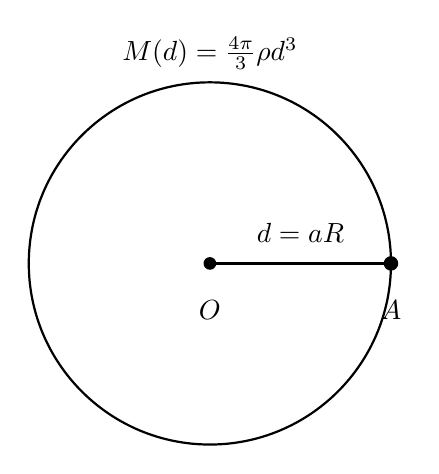
\begin{tikzpicture}[scale=1.15]
\draw[thick] (0,0) circle (2);
\fill (0,0) circle (0.07);
\fill (2,0) circle (0.08);
\draw[thick] (0,0) -- (2,0);
\draw (1,0.12) node[above] {\(d=aR\)};
\draw (0,-0.3) node[below] {\(O\)};
\draw (2,-0.3) node[below] {\(A\)};
\draw (0,2.32) node {\(M(d)=\frac{4\pi}{3}\rho d^3\)};
\end{tikzpicture}
\caption{Phép quy giản Newton. Đối với gia tốc của thiên hà \(A\), các lớp vỏ bên ngoài triệt tiêu nhau và khối lượng bên trong bán kính \(d\) tác dụng như thể tập trung tại \(O\).}
\label{fig:c01-newton-sphere}
\end{figure}

Đối với một phân bố khối lượng đối xứng cầu, lực tổng do vật chất ở ngoài mặt cầu đi qua \(A\) gây ra bằng không. Vật chất bên trong tác dụng như thể được tập trung tại tâm. Khối lượng bị bao chứa là
\begin{equation}
M(d)=\frac{4\pi}{3}\rho d^3.
\label{eq:c01-enclosed-mass}
\end{equation}
Khi đó định luật nghịch đảo bình phương của Newton cho gia tốc của \(A\):
\begin{equation}
\ddot d=-\frac{GM(d)}{d^2}.
\end{equation}
Dùng phương trình~\eqref{eq:c01-radial-kinematics},
\begin{align}
\ddot a R
&=-\frac{G}{d^2}\left(\frac{4\pi}{3}\rho d^3\right) \\
&=-\frac{4\pi G}{3}\rho d \\
&=-\frac{4\pi G}{3}\rho aR.
\end{align}
Bán kính đồng chuyển động triệt tiêu, còn lại
\begin{equation}
\boxed{\frac{\ddot a}{a}=-\frac{4\pi G}{3}\rho.}
\label{eq:c01-acceleration}
\end{equation}
Sự triệt tiêu này là phép kiểm tra tính nhất quán. Mọi thiên hà đồng chuyển động, bất kể \(R\), đều tuân theo cùng một phương trình cho cùng một thừa số tỉ lệ.

Thế phương trình~\eqref{eq:c01-density-dilution} vào ta được một trong hai dạng tương đương
\begin{equation}
\frac{\ddot a}{a}=-\frac{4\pi G\nu}{3a^3},
\qquad
\ddot a=-\frac{4\pi G\nu}{3a^2}.
\label{eq:c01-acceleration-nu}
\end{equation}
Dạng thứ nhất cho thấy gia tốc tương đối; dạng thứ hai tách riêng \(\ddot a\). Việc giữ \(a\) ở vế trái là một quy ước, không phải là thay đổi vật lý.

\begin{classroomqa}
\audiencequestion{Gốc là tùy ý, vậy mà mọi lực trong phép tính đều hướng về đó. Làm sao một lựa chọn gốc khác lại cho cùng một vũ trụ?}
\lecturerresponse{Phương trình nói về chuyển động tương đối. Lặp lại phép tính quanh bất kỳ thiên hà nào khác cũng cho cùng một phương trình, vì tính đồng nhất khiến khối lượng bị bao chứa chỉ phụ thuộc vào bán kính vật lý. Nếu ta biến đổi sang một hệ quy chiếu gia tốc gắn với một thiên hà khác mà vẫn giữ các lực được quy về gốc thứ nhất, thì cũng phải đưa thêm lực quán tính tương ứng vào. Chọn một hệ nghỉ trung tâm chỉ đơn thuần tránh phải mang theo phần hạch toán phụ thêm ấy. Kết quả bất biến là phương trình~\eqref{eq:c01-acceleration}, không phải một tâm đặc biệt. \lecturetimestamp{00:43:56--00:46:58}}
\end{classroomqa}

\begin{classroomqa}
\audiencequestion{Kết quả đó còn đúng nếu mật độ khối lượng đồng chuyển động \(\nu\) thay đổi theo vị trí không?}
\lecturerresponse{Không phải dưới dạng chỉ với một hàm này. Sự triệt tiêu gọn gàng phụ thuộc vào \(M\propto d^3\) với cùng một hệ số tỉ lệ ở khắp mọi nơi. Nếu \(\nu\) biến thiên đáng kể trên thang lấy trung bình, các vùng khác nhau sẽ đòi hỏi những động lực học cục bộ khác nhau và một thừa số tỉ lệ đồng nhất duy nhất sẽ không còn mô tả được chúng nữa. Tính đồng nhất là điều cốt yếu ở đây. \lecturetimestamp{00:47:05--00:47:51}}
\end{classroomqa}

\begin{classroomqa}
\audiencequestion{Vì sao viết \(\ddot a/a\) thay vì chuyển thừa số \(a\) sang vế phải?}
\lecturerresponse{Cả hai dạng đều đúng. Trong vũ trụ học, theo quy ước người ta viết gia tốc tương đối \(\ddot a/a\), một phần vì có thể so sánh trực tiếp với tốc độ giãn nở tương đối \(H=\dot a/a\). Nhân cả phương trình với \(a\) cho phương trình vi phân y hệt. \lecturetimestamp{00:50:36--00:51:29}}
\end{classroomqa}

Phương trình~\eqref{eq:c01-acceleration} ngay lập tức loại trừ một vũ trụ Newton đồng nhất tĩnh chứa đầy vật chất thông thường. Một thừa số tỉ lệ không đổi sẽ có \(\ddot a=0\), trong khi mật độ dương làm cho vế phải âm. Điều này \emph{không} cho ta biết vũ trụ đang giãn nở hay co lại. Nó chỉ cho ta biết dấu của gia tốc.

\section{Gia tốc âm không có nghĩa là co lại}

Sự phân biệt giữa vận tốc và gia tốc là sơ đẳng nhưng có tính quyết định. Một chiếc Ferrari đang chạy về phía trước trên Autobahn có thể có vận tốc dương trong khi đang phanh với gia tốc âm. Tương tự, một vũ trụ có thể có
\begin{equation}
\dot a>0,
\qquad
\ddot a<0:
\end{equation}
nghĩa là nó đang giãn nở, nhưng tốc độ giãn nở đang giảm.

Để quyết định xem chuyển động có cuối cùng đảo chiều hay không, hãy so sánh bài toán vũ trụ học với một hạt thử chuyển động theo phương xuyên tâm trong trường hấp dẫn của Trái Đất. Bây giờ gọi \(x\) là khoảng cách vật lý của hạt tới một khối lượng trung tâm \(M\); nó không liên quan đến tọa độ đồng chuyển động trước đó. Phương trình Newton là
\begin{equation}
\ddot x=-\frac{GM}{x^2}.
\label{eq:c01-particle-force}
\end{equation}
Gia tốc luôn hướng vào trong. Tuy vậy, một hạt được ném ra ngoài vẫn có thể tiếp tục đi ra ngoài trong một thời gian dài, hoặc mãi mãi. Một hạt đã chuyển động vào trong sẽ có vận tốc ngày càng âm. Chỉ riêng định luật lực không quyết định chuyển động nào xảy ra; điều đó do điều kiện đầu quyết định.

\begin{classroomqa}
\audiencequestion{Liệu \(\ddot a<0\) có nghĩa là vũ trụ đang co lại không?}
\lecturerresponse{Không. Co lại có nghĩa là \(\dot a<0\). \(\ddot a\) âm chỉ có nghĩa là \(\dot a\) giảm theo thời gian. Nếu \(\dot a\) ban đầu dương, hấp dẫn làm chậm sự giãn nở; việc nó có đạt tới 0 hay không phụ thuộc vào tốc độ giãn nở ban đầu, đúng hệt như số phận của một vật phóng ra ngoài phụ thuộc vào việc nó nhỏ hơn hay lớn hơn vận tốc thoát. \lecturetimestamp{00:51:30--00:56:18}}
\end{classroomqa}

\begin{figure}[ht]
\centering
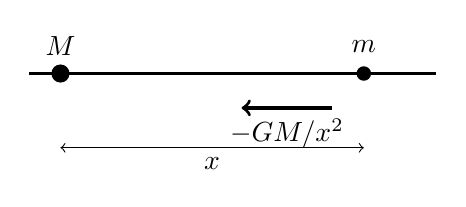
\begin{tikzpicture}[scale=1.15]
\fill (0,0) circle (0.1);
\draw (0,0.3) node {\(M\)};
\draw[thick] (-0.35,0) -- (4.15,0);
\fill (3.35,0) circle (0.08);
\draw (3.35,0.3) node {\(m\)};
\draw[->,very thick] (3.0,-0.38) -- (2.0,-0.38)
  node[midway,below] {\(-GM/x^2\)};
\draw[<->] (0,-0.82) -- (3.35,-0.82)
  node[midway,below] {\(x\)};
\end{tikzpicture}
\caption{Bài toán một hạt theo phương xuyên tâm được dùng để tách dấu của gia tốc khỏi hướng và kết cục của chuyển động.}
\label{fig:c01-particle-sketch}
\end{figure}

Năng lượng làm cho các khả năng trở nên rõ ràng. Cơ năng bảo toàn là
\begin{equation}
E=\frac12 m\dot x^{\,2}-\frac{GMm}{x}.
\label{eq:c01-particle-energy}
\end{equation}
Thế năng tỉ lệ với \(1/x\), không phải \(1/x^2\); lấy đạo hàm \(-GMm/x\) sẽ cho lực nghịch đảo bình phương.

\begin{figure}[ht]
\centering
\includegraphics[width=0.82\textwidth]{lecture_01_figure_02.png}
\caption{Bảng ở đầu lập luận năng lượng: một khối lượng thử đang chuyển động và hạng động năng của nó, ngay trước khi thế năng hấp dẫn được đưa trở lại.}
\lectureframe{00:58:57}
\end{figure}

Nếu \(E<0\), một hạt đang chuyển động ra ngoài không thể đạt tới vô cực, nơi thế năng của nó tiến tới 0 và động năng của nó không âm. Nó phải dừng lại tại một \(x\) hữu hạn rồi quay trở lại. Nếu \(E>0\), nó không thể dừng lại, vì tại một điểm ngoặt động năng sẽ triệt tiêu và thế năng còn lại sẽ âm, mâu thuẫn với việc bảo toàn một \(E\) dương. Ranh giới là
\begin{equation}
E=0,
\end{equation}
từ đó xác định vận tốc thoát:
\begin{equation}
\frac12 m v_{\rm esc}^2-\frac{GMm}{x}=0,
\qquad
\boxed{v_{\rm esc}^2=\frac{2GM}{x}.}
\label{eq:c01-escape-velocity}
\end{equation}

\begin{figure}[ht]
\centering
\includegraphics[width=0.88\textwidth]{lecture_01_figure_03.png}
\caption{Ranh giới năng lượng bằng 0 đang thành hình trên bảng. Các phương trình gia tốc vũ trụ học ở trước vẫn được đóng khung bên trái, trong khi bài toán thoát theo phương xuyên tâm được triển khai ở bên phải.}
\lectureframe{01:01:37}
\end{figure}

Ngay ở vận tốc thoát, hạt chậm dần mãi mãi. Tốc độ của nó chỉ tiến về 0 khi \(x\to\infty\); nó không bao giờ đạt tới một điểm ngoặt hữu hạn. Trường hợp biên này sẽ là mô hình vũ trụ học đơn giản nhất.

\section{Phương trình năng lượng vũ trụ học}

Quay lại xét một thiên hà ở bán kính đồng chuyển động cố định \(R\). Theo định lý vỏ cầu, chuyển động xuyên tâm của nó giống hệt chuyển động của một hạt chuyển động bên ngoài một khối lượng điểm bằng khối lượng nằm trong khối cầu đồng chuyển động của nó.

\begin{figure}[ht]
\centering
\includegraphics[width=0.82\textwidth]{lecture_01_figure_04.png}
\caption{Hình phác họa lực nghịch đảo bình phương và hạt xuyên tâm được dùng khi đưa lập luận năng lượng của bài toán một hạt trở lại vũ trụ học.}
\lectureframe{01:04:14}
\end{figure}

Khối lượng bị bao chứa không tăng khi khối cầu vật lý giãn nở. Khối cầu ấy là đồng chuyển động, nên nó luôn chứa cùng những thiên hà đó:
\begin{align}
M
&=\frac{4\pi}{3}\rho(aR)^3 \\
&=\frac{4\pi}{3}\frac{\nu}{a^3}a^3R^3 \\
&=\frac{4\pi}{3}\nu R^3.
\label{eq:c01-fixed-enclosed-mass}
\end{align}
Biểu thức thứ nhất chỉ có vẻ phụ thuộc thời gian cho đến khi ta tính đến sự làm loãng mật độ. Các thừa số \(a^3\) triệt tiêu nhau.

\begin{classroomqa}
\audiencequestion{Khi mặt cầu giãn nở, nó có bao chứa nhiều khối lượng hơn không?}
\lecturerresponse{Không. Bán kính vật lý của nó tăng lên, nhưng biên đồng chuyển động của nó chuyển động cùng các thiên hà. Không có vật chất nào đi qua biên đó trong dòng chảy đồng nhất lý tưởng, và phương trình~\eqref{eq:c01-fixed-enclosed-mass} cho thấy sự triệt tiêu ấy một cách tường minh. \lecturetimestamp{01:04:37--01:05:20}}
\end{classroomqa}

Vận tốc vật lý của thiên hà là \(\dot d=\dot a R\), và khoảng cách của nó tới gốc tọa độ được chọn là \(d=aR\). Vì vậy, năng lượng Newton được bảo toàn của nó là
\begin{equation}
\boxed{
E=\frac12 m\dot a^{\,2}R^2-\frac{GMm}{aR}.
}
\label{eq:c01-cosmological-energy}
\end{equation}

\begin{figure}[ht]
\centering
\includegraphics[width=0.82\textwidth]{lecture_01_figure_05.png}
\caption{Các hạng động năng và thế năng vũ trụ học trên bảng. Mẫu số đầy đủ \(aR\) trong phương trình~\eqref{eq:c01-cosmological-energy} suy ra từ bán kính vật lý và phép suy dẫn đi kèm.}
\lectureframe{01:06:12}
\end{figure}

Ba trường hợp năng lượng của hạt trở thành ba trường hợp vũ trụ học:
\begin{description}[style=nextline]
\item[\(E<0\):] sự giãn nở ban đầu nhỏ hơn vận tốc thoát; \(a(t)\) đạt cực đại và vũ trụ co sụp trở lại.
\item[\(E=0\):] vũ trụ đúng tới hạn; sự giãn nở chậm lại mãi mãi và chỉ tiệm cận đến tốc độ bằng không.
\item[\(E>0\):] sự giãn nở ban đầu lớn hơn vận tốc thoát; trong mô hình Newton, vũ trụ giãn nở mãi mãi với vận tốc lùi xa tiệm cận khác không.
\end{description}

Ta bắt đầu với trường hợp biên \(E=0\). Đặt phương trình~\eqref{eq:c01-cosmological-energy} bằng không, khử \(m\), và chia cho \(a^2R^2/2\), ta được
\begin{align}
\frac12\dot a^{\,2}R^2&=\frac{GM}{aR}, \\
\left(\frac{\dot a}{a}\right)^2&=\frac{2GM}{a^3R^3}.
\label{eq:c01-energy-intermediate}
\end{align}
Vì
\begin{equation}
\rho=\frac{M}{(4\pi/3)a^3R^3},
\end{equation}
phương trình~\eqref{eq:c01-energy-intermediate} trở thành
\begin{equation}
\boxed{
H^2=\left(\frac{\dot a}{a}\right)^2=\frac{8\pi G}{3}\rho.
}
\label{eq:c01-first-friedmann}
\end{equation}
Đây là phương trình Friedmann thứ nhất cho một vũ trụ phẳng theo không gian, chỉ gồm vật chất và có hằng số vũ trụ bằng không, được suy ra ở đây từ định luật bảo toàn năng lượng Newton.

\begin{classroomqa}
\classquestion{Một hạt được phóng đi đúng bằng vận tốc thoát thì điều gì xảy ra?}
\lecturerresponse{Nó chậm dần mà không bao giờ đảo chiều. Tốc độ của nó chỉ tiến về không ở khoảng cách vô hạn. Vũ trụ có năng lượng bằng không cũng hành xử theo cách đó: \(H\) giảm, nhưng \(\dot a\) vẫn dương và không có sự quay đầu nào xảy ra trong thời gian hữu hạn. \lecturetimestamp{01:10:45--01:12:10}}
\end{classroomqa}

Các hệ số \(4\pi/3\) và \(8\pi G/3\) không phải là những chi tiết trang trí tùy tiện. \(4\pi/3\) là thể tích của một mặt cầu, còn hệ số hai đến từ động năng. Trong thuyết tương đối rộng, chính \(8\pi G\) ấy xuất hiện trong phương trình trường Einstein, và thành phần thời-gian–thời-gian của nó dẫn tới phương trình Friedmann tương đối tính. Sự trùng hợp đó không phải ngẫu nhiên, nhưng phép suy dẫn hiện tại vẫn chưa bao gồm áp suất, độ cong không gian xét như hình học, hay hằng số vũ trụ.

\section{Nghiệm tới hạn do vật chất chi phối}

Dùng định luật mật độ \(\rho=\nu/a^3\) trong phương trình~\eqref{eq:c01-first-friedmann}:
\begin{equation}
\left(\frac{\dot a}{a}\right)^2=\frac{8\pi G\nu}{3a^3}.
\label{eq:c01-matter-friedmann}
\end{equation}
Hằng số \(\nu\) phụ thuộc vào phép chuẩn hóa tùy ý của các tọa độ đồng chuyển động. Để làm lộ ra sự phụ thuộc theo thời gian, đặt
\begin{equation}
K\equiv\frac{8\pi G\nu}{3}>0.
\end{equation}
Khi đó
\begin{equation}
\dot a^{\,2}=\frac{K}{a}.
\label{eq:c01-normalized-friedmann}
\end{equation}

\begin{figure}[ht]
\centering
\includegraphics[width=0.76\textwidth]{lecture_01_figure_06.png}
\caption{Dạng tỉ lệ Friedmann do vật chất chi phối trên bảng: trước hết viết kèm các hằng số của nó, rồi sau đó làm lộ rõ lũy thừa nghịch cốt yếu của hệ số tỉ lệ.}
\lectureframe{01:14:44}
\end{figure}

Vế phải của phương trình~\eqref{eq:c01-normalized-friedmann} dương với mọi \(a\) hữu hạn dương. Một sự quay đầu sẽ đòi hỏi \(\dot a=0\), nên vũ trụ tới hạn không bao giờ quay đầu. Đà giãn nở của nó suy yếu đều đặn, nhưng không bao giờ suy yếu đến mức dừng lại.

Bây giờ hãy giải phương trình. Ta có thể tách biến trực tiếp,
\begin{equation}
a^{1/2}\,da=\sqrt{K}\,dt,
\end{equation}
hoặc theo bài giảng mà thử một luật lũy thừa,
\begin{equation}
a(t)=Ct^p.
\label{eq:c01-power-trial}
\end{equation}
Khi đó
\begin{equation}
\frac{\dot a}{a}=\frac{p}{t},
\qquad
\frac{K}{a^3}=\frac{K}{C^3t^{3p}}.
\end{equation}
Thế vào phương trình~\eqref{eq:c01-matter-friedmann} cho
\begin{equation}
\frac{p^2}{t^2}=\frac{K}{C^3t^{3p}}.
\end{equation}
So khớp các số mũ và các hệ số thu được
\begin{equation}
3p=2,
\qquad
C^3=\frac{K}{p^2}=\frac{9K}{4}.
\end{equation}
Do đó
\begin{equation}
\boxed{
a(t)=\left(\frac{3\sqrt K}{2}t\right)^{2/3}\propto t^{2/3}.
}
\label{eq:c01-two-thirds}
\end{equation}
Mốc thời gian đã được chọn sao cho \(a=0\) tại \(t=0\). Tổng quát hơn, có thể thay \(t\) bằng \(t-t_0\).

Hệ số tỉ lệ tăng mãi mãi, còn
\begin{equation}
\dot a\propto t^{-1/3}\longrightarrow0,
\qquad
H=\frac{2}{3t}\longrightarrow0.
\label{eq:c01-asymptotic-slope}
\end{equation}
Đồ thị của nó luôn tăng và luôn lõm xuống. Nó không tiến đến một đường ngang nào vì chính \(a(t)\) không bị chặn trên, nhưng độ dốc của nó tiến về không.

\begin{classroomqa}
\audiencequestion{Có phải \(t^{2/3}\) chỉ được tìm thấy vì dạng thử đó tình cờ cho kết quả không? Liệu một dạng thử khác có thể cho một nghiệm năng lượng bằng không khác không?}
\lecturerresponse{Dạng thử xác định nghiệm chứ không chỉ nêu ra một khả năng. Phương trình bậc nhất của nhánh giãn nở \(\dot a=\sqrt{K/a}\) tích phân được một cách duy nhất, trừ phép chuẩn hóa và việc chọn gốc thời gian, thành \(a\propto(t-t_0)^{2/3}\). Những năng lượng toàn phần khác nhau cho những phương trình vi phân khác nhau và vì thế những lịch sử vũ trụ học khác nhau. \lecturetimestamp{01:27:07--01:27:43}}
\end{classroomqa}

\begin{classroomqa}
\audiencequestion{Rốt cuộc đường cong tới hạn có trở nên nằm ngang không?}
\lecturerresponse{Độ dốc của nó tiến về không: \(\dot a\propto t^{-1/3}\). Tuy vậy, nó vẫn dương ở mọi thời điểm hữu hạn, nên hệ số tỉ lệ tiếp tục tăng mà không bị chặn. Vũ trụ tiệm cận trạng thái nghỉ mà không bao giờ đạt tới nó. \lecturetimestamp{01:27:48--01:28:57}}
\end{classroomqa}

Kết quả đơn giản này thật nổi bật về mặt lịch sử. Newton đã có trong tay cơ học và định lý vỏ cầu cần cho phép suy dẫn này, và ông đã xem xét những câu hỏi về một vũ trụ hấp dẫn vô hạn, nhưng ông đã không xây dựng mô hình giãn nở. Cuộc thảo luận trên lớp gợi ý rằng những cam kết triết học và thần học về lịch sử vũ trụ có thể đã ảnh hưởng đến việc những câu hỏi nào dường như tự nhiên đối với ông. Gợi ý lịch sử ấy không phải là một phần của phép suy dẫn; điểm toán học duy nhất là các công cụ Newton cần thiết đã sẵn có.

\begin{classroomqa}
\audiencequestion{Cách xây dựng Newton này có giả định một vũ trụ vô hạn không?}
\lecturerresponse{Nó giả định không gian Newton Euclid, phẳng theo không gian. Trong mô hình Newton thông thường, không gian đó kéo dài vô hạn, nên mô hình là vô hạn về mặt không gian ngay cả khi các khoảng cách giữa các thiên hà đồng chuyển động thay đổi theo thời gian. Các hình học không gian cong hữu hạn thuộc về cách xử lý tương đối tính. \lecturetimestamp{01:22:12--01:22:55}}
\end{classroomqa}

\section{Vượt ra ngoài mô hình năng lượng không}

Trường hợp năng lượng không là một sự đơn giản hóa có chủ ý, không phải vũ trụ Newton duy nhất. Giữ \(E\neq0\) trong phương trình~\eqref{eq:c01-cosmological-energy} ta được
\begin{equation}
\left(\frac{\dot a}{a}\right)^2
=\frac{8\pi G}{3}\rho+\frac{2E}{mR^2a^2}.
\label{eq:c01-nonzero-energy}
\end{equation}
Tính đồng nhất đòi hỏi tổ hợp \(2E/(mR^2)\) phải như nhau đối với mọi mặt cầu đồng chuyển động đại diện. Viết nó thành hằng số \(C_E\),
\begin{equation}
H^2=\frac{8\pi G}{3}\rho+\frac{C_E}{a^2}.
\end{equation}
\(C_E\) dương tương ứng với năng lượng cao hơn mức thoát; \(C_E\) âm cho phép một sự quay đầu. Trong ký hiệu tương đối tính, hạng năng lượng này được diễn giải lại thông qua độ cong không gian, một mối liên hệ sẽ để dành cho phần trình bày sau.

Cả ba lịch sử chỉ có vật chất đều có gia tốc âm chừng nào vật chất còn chi phối:
\begin{equation}
\ddot a=-\frac{4\pi G}{3}\rho a<0.
\end{equation}
Đường cong co sụp trở lại đi lên, đạt \(\dot a=0\), rồi đi xuống. Đường cong tới hạn \(t^{2/3}\) đi lên mãi mãi với độ dốc tiến về không. Đường cong năng lượng dương cũng đi lên mãi mãi và tiến gần tới tăng trưởng tuyến tính. Một phác họa tạm thời trên bảng về các trường hợp này đã được chỉnh lại trong buổi giảng; kết luận vững chắc là tính lõm xuống chung của chúng, chứ không phải mọi chi tiết của phác họa đầu tiên.

Vũ trụ quan sát được còn làm nhiều hơn thế. Sự giãn nở thời kỳ đầu do vật chất chi phối của nó được xấp xỉ khá tốt bằng một đường cong giảm tốc, nhưng ở thời muộn đường cong ấy bẻ cong lên trên:
\begin{equation}
\ddot a>0.
\end{equation}
Vật chất thông thường không áp suất không thể tạo ra dấu đó trong phương trình~\eqref{eq:c01-acceleration}. Cần có một hạng bổ sung. Trong mô hình hiện đại đơn giản nhất, đó là một hằng số vũ trụ; tổng quát hơn, nó được gọi là năng lượng tối. Chương hiện tại cố ý bỏ qua nó để trước hết có thể hiểu một cách sáng sủa động lực học vật chất Newton.

\begin{classroomqa}
\audiencequestion{Liệu \(8\pi G\) trong phương trình Friedmann có phải chính là hệ số xuất hiện trong phương trình trường Einstein không, và chúng ta đã đưa vào hằng số vũ trụ chưa?}
\lecturerresponse{Cùng một hệ số chuẩn hóa hấp dẫn xuất hiện trong thuyết tương đối rộng, và phương trình trường ở thành phần thời-gian–thời-gian tái tạo phương trình Friedmann tương đối tính. Mô hình ở đây không chứa hằng số vũ trụ. Đây là một vũ trụ do vật chất chi phối; hạng hằng số vũ trụ còn thiếu chính là loại hạng có thể giải thích gia tốc ở thời muộn. \lecturetimestamp{01:30:15--01:31:06}}
\end{classroomqa}

\section{Dòng chảy trung bình và các lệch cục bộ}

Sự giãn nở đồng nhất là một mô tả ở mức thô. Nó không nói rằng mọi vật thể đều đi xa khỏi mọi láng giềng gần của nó. Những hệ bị liên kết bởi hấp dẫn hoặc bằng cách khác có thể tách khỏi dòng Hubble. Chẳng hạn, Ngân Hà và Andromeda đang tiến lại gần nhau chứ không tuân theo định luật lùi xa ở quy mô lớn.

Độ lệch của vận tốc một thiên hà riêng lẻ so với dòng Hubble được gọi là \emph{vận tốc riêng} của nó. Thuật ngữ này là thuật ngữ kỹ thuật, không phải một sự phán xét về thiên hà đó. Định luật Hubble trở thành một gần đúng tốt hơn khi ta lấy trung bình trên những khoảng cách lớn hơn và những thể tích lớn hơn. Ở thang của một thiên hà liên kết hấp dẫn, một cụm, hay một vùng quá đậm đặc cục bộ, các lực cục bộ có thể chi phối sự giãn nở nền.

\begin{classroomqa}
\audiencequestion{Có phải một số vùng vẫn có thể co lại mặc dù nhìn chung vũ trụ đang giãn nở không?}
\lecturerresponse{Chắc chắn là có. Các hệ liên kết và những thăng giáng đủ đậm đặc không nhất thiết phải tuân theo sự giãn nở trung bình. Hệ Ngân Hà--Andromeda là một ví dụ quen thuộc. Trong một phép tính vũ trụ học, người ta lấy trung bình trên những thể tích đủ lớn để các chuyển động riêng và các thăng giáng mật độ cục bộ này không chi phối; khi đó \(a(t)\) thu được mô tả nền, chứ không phải mọi cặp vật thể. \lecturetimestamp{01:31:00--01:34:13}}
\end{classroomqa}

Sự tương tự ở đây là một chất khí thông thường. Nói rằng không khí trong một căn phòng là đồng đều không có nghĩa là phủ nhận các thăng giáng phân tử hay các biến thiên mật độ cục bộ. Điều ấy chỉ nói rằng các giá trị trung bình trên những vùng đủ lớn là ổn định. Tính đồng nhất vũ trụ có cùng vị thế lôgic như vậy, dù ở những thang đo lớn hơn vô cùng nhiều. Một vùng hình thành với mật độ nhỉnh hơn trung bình một chút có thể có đủ tự hấp dẫn để chống lại sự giãn nở và cuối cùng sụp đổ thành một cấu trúc liên kết.

\begin{classroomqa}
\audiencequestion{Liệu quan sát có thể quyết định xem các thiên hà chuyển động trong không gian hay chính không gian giãn nở làm chúng tách xa nhau hay không?}
\lecturerresponse{Không thể, khi hai cách mô tả gán cùng một khoảng cách \(d_{AB}(t)\) cho mọi cặp. Một cách mô tả để các thiên hà chuyển động trên một nền tọa độ trông như cố định; cách mô tả đồng chuyển động giữ các thiên hà cố định và để thừa số tỉ lệ đảm nhận sự thay đổi đó. Chúng tương đương về mặt toán học. Thuyết tương đối rộng khiến lối diễn đạt thứ hai tự nhiên hơn, nhưng trong phép so sánh này nó không tạo ra một đại lượng quan sát được riêng biệt. \lecturetimestamp{01:34:14--01:34:59}}
\end{classroomqa}

\begin{classroomqa}
\audiencequestion{Ngoài độ sáng của siêu tân tinh loại Ia, còn có bằng chứng độc lập nào về sự gia tốc của vũ trụ không?}
\lecturerresponse{Có. Suy luận này đến từ một mạng lưới các quan sát, đặc biệt là từ cách các phép đo siêu tân tinh và bức xạ nền vi sóng vũ trụ ăn khớp với nhau. Không có một dữ liệu đơn lẻ nào gánh toàn bộ kết luận; điểm quan trọng là tính nhất quán giữa các phép đo vũ trụ học độc lập. \lecturetimestamp{01:35:00--01:35:38}}
\end{classroomqa}

\section{Những gì đã được xác lập}

Lập luận đã được triển khai theo một trình tự chặt chẽ:
\begin{enumerate}
\item Tính đẳng hướng ở quy mô lớn, cùng với việc bác bỏ một tâm đặc biệt, gợi ý tính đồng nhất.
\item Tính đồng nhất cho phép một lưới đồng chuyển động với một thừa số tỉ lệ \(a(t)\).
\item Lấy đạo hàm theo thời gian của khoảng cách vật lý suy ra định luật Hubble,
  \[
  H=\frac{\dot a}{a},
  \qquad
  v=Hd.
  \]
\item Bảo toàn khối lượng trong một ô đồng chuyển động cho
  \[
  \rho=\frac{\nu}{a^3}.
  \]
\item Định lý vỏ cầu của Newton cho phương trình gia tốc
  \[
  \frac{\ddot a}{a}=-\frac{4\pi G}{3}\rho.
  \]
\item Năng lượng bảo toàn phân loại sự giãn nở thành các trường hợp tái co sụp, tới hạn và không bị ràng buộc.
\item Khi tổng năng lượng bằng không,
  \[
  H^2=\frac{8\pi G}{3}\rho,
  \qquad
  a(t)\propto t^{2/3}.
  \]
\end{enumerate}

Đây là một mô hình Newton hoàn chỉnh cho trường hợp vật chất chi phối, nhưng chưa phải là một mô tả hoàn chỉnh về vũ trụ của chúng ta. Nó nắm bắt được lôgic giảm tốc ban đầu, cho thấy vì sao một vũ trụ đồng nhất được lấp đầy không thể duy trì trạng thái tĩnh, và xác định sự giãn nở tới hạn ở ngưỡng thoát. Năng lượng khác không, hình học không gian tương đối tính, áp suất, bức xạ và hạng tử chịu trách nhiệm cho gia tốc muộn vẫn còn phải được bổ sung.
